Die nachfolgende Grafik \ref{pic:01_projektablauf} zeigt den neuen Projektablauf 
mit einer Aufteilung in vier Hauptabschnitte. Jedem Abschnitt wurden Resultate
hinzugefügt, die während dieser Phase erarbeitet oder durchgeführt werden sollen.

\begin{figure}[htbp]
\begin{center}
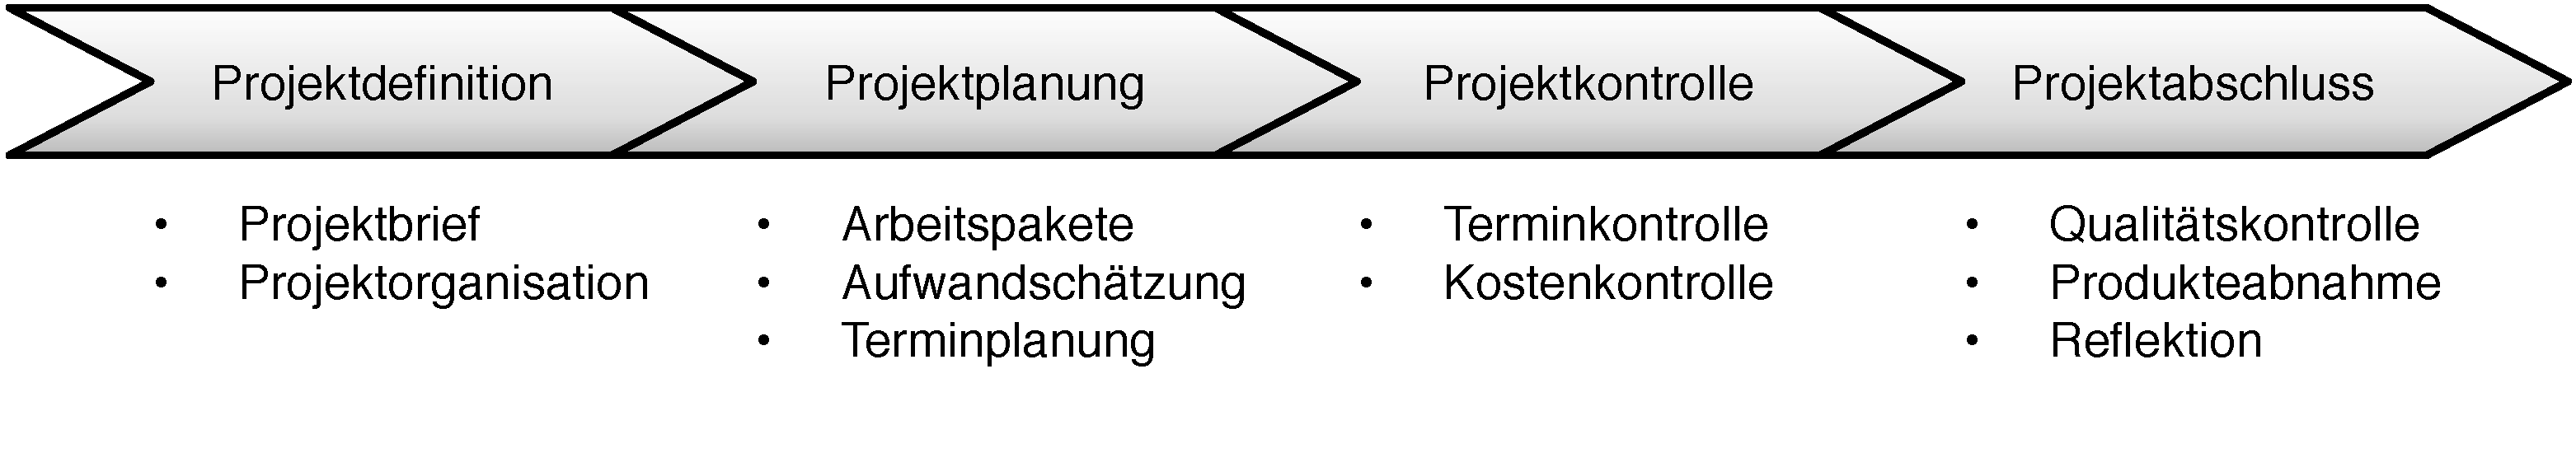
\includegraphics[width=0.99\textwidth,angle=0]{./bilder/loesung/01_projektablauf.pdf}
\caption[Aufteilung des Projektablaufes mit Resultaten]{Aufteilung des Projektablaufes mit Resultaten\footnotemark}
\label{pic:01_projektablauf}
\end{center}
\end{figure}
\footnotetext{Eigene Darstellung}

In den folgenden Kapiteln wird einzeln auf die vier Hauptabschnitte und deren
Resultate eingegangen. Es wird aufgezeigt, wie die jeweils erwarteten Resultate 
erarbeitet werden sollen.

Zusätzlich werden die Stellen hervorgehoben, wo der Einsatz und die Verwendung 
von Instrumenten sinnvoll ist. Die Wahl dieser Instrumente wird später in einem
separaten Kapitel \ref{chap:instrumentenwahl} behandelt. Zum besseren Verständnis
wird an den jeweiligen Stellen das nötigen Instrument mit einer fortlaufenden
Nummer (\textbf{AI}n) versehen. So kann darauf im separaten Kapitel wieder Bezug 
genommen werden.

\newcounter{icounter}
\subsection{Projektdefinition}
In der Grafik \ref{pic:02_01_projektdefinition} ist der Ablauf der Projektdefinition 
ersichtlich. Die potenziellen Projekte (\textbf{0}) gelangen weiterhin zu den
Partnern (\textbf{1.1}), die entscheiden ob ein Projekt angenommen werden soll
oder nicht (\textbf{1.2}). Im Falle einer Absage, wird das dem Kunden von einem
Partner mitgeteilt (\textbf{2.1} bis \textbf{2.3}).

Wird das Projekt angenommen, bestimmen die Partner einen Hauptverantwortlichen
Partner und einen Verantwortlichen Projektleiter (\textbf{3.1}). Der Projektleiter
erstellt darauf den Projektbrief (\textbf{3.2}) und danach kümmert er sich um
die Projektorganisation (\textbf{3.3}).

\begin{figure}[htbp]
\begin{center}
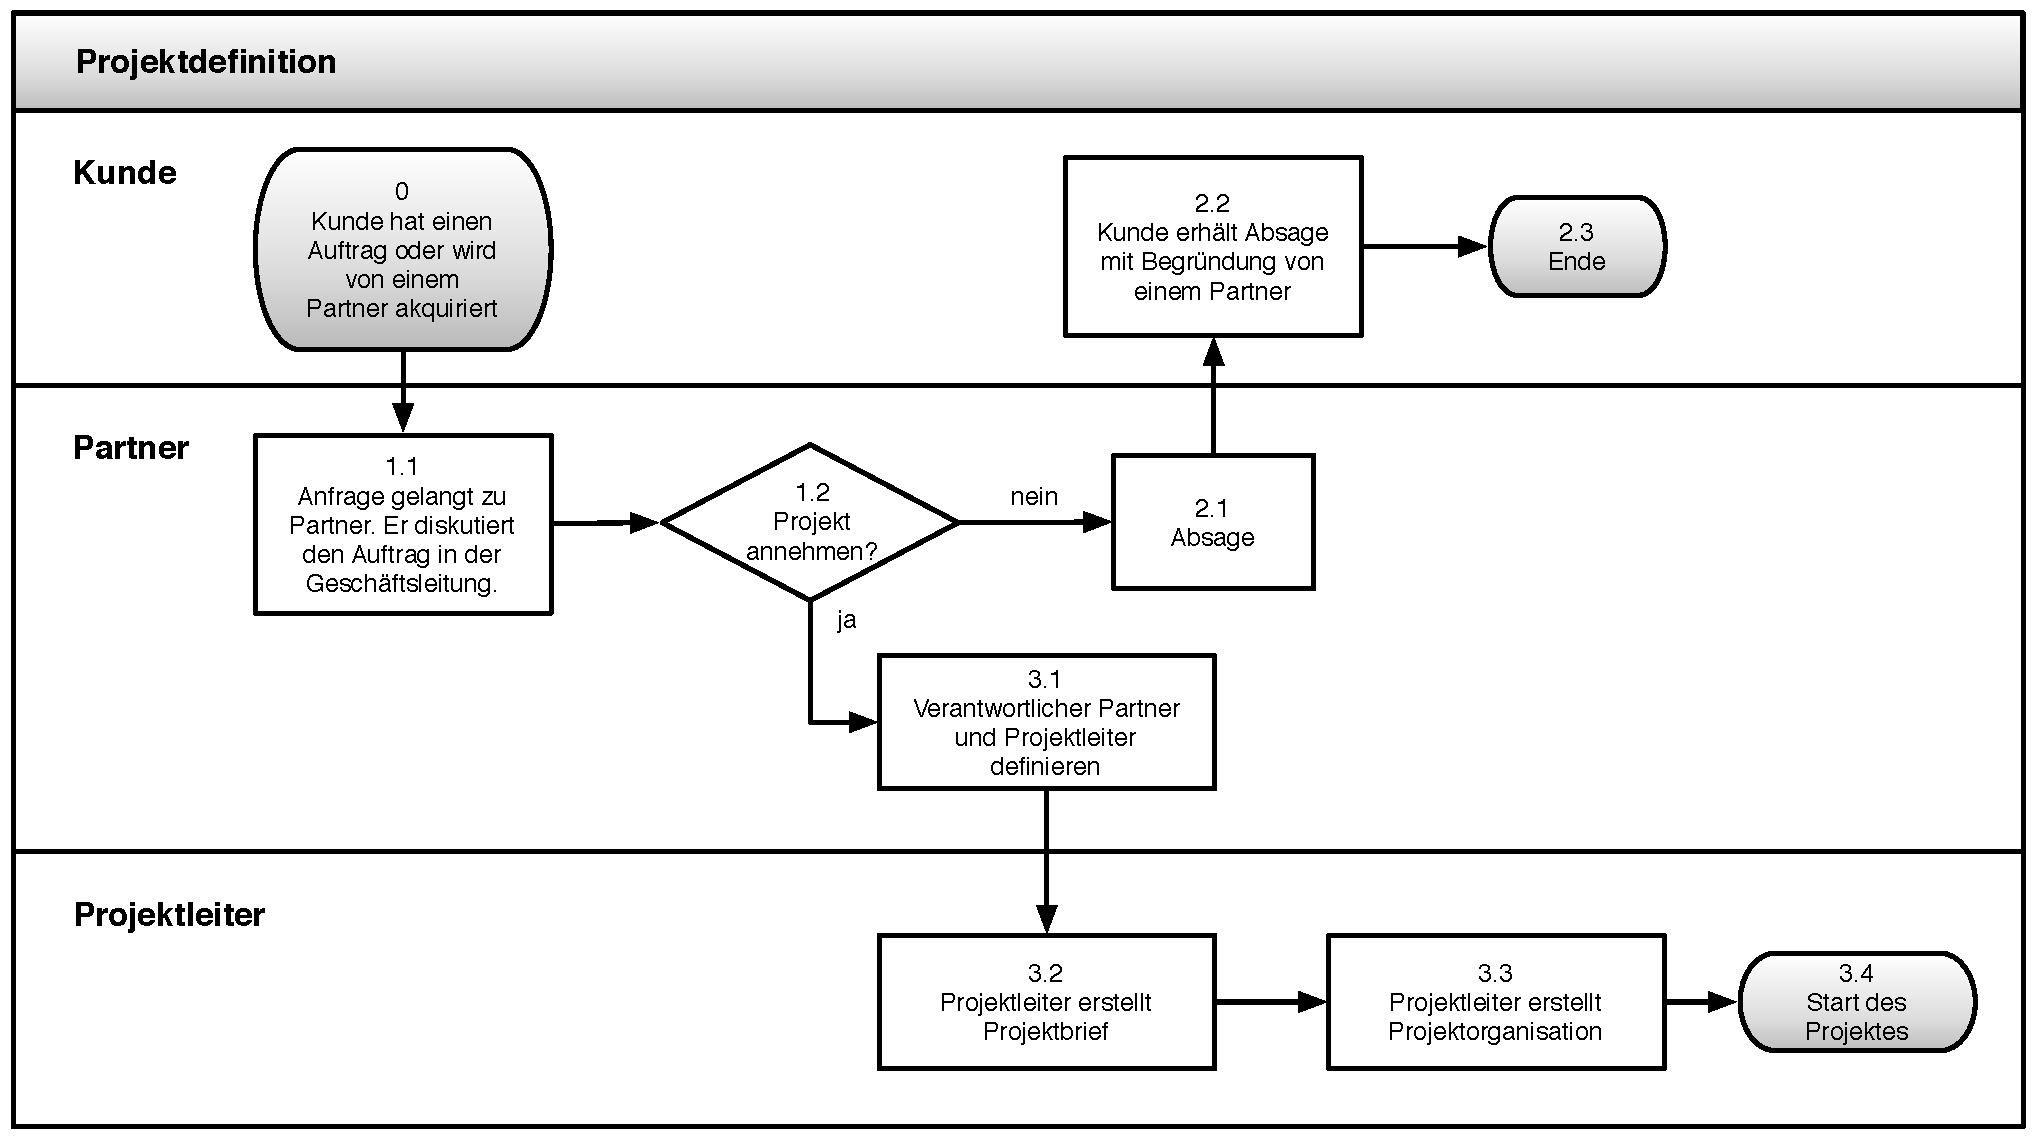
\includegraphics[width=0.99\textwidth,angle=0]{./bilder/loesung/02_01_projektdefinition.pdf}
\caption[Ablauf der Projektdefinitionsphase]{Ablauf der Projektdefinitionsphase\footnotemark}
\label{pic:02_01_projektdefinition}
\end{center}
\end{figure}
\footnotetext{Eigene Darstellung}

\subsubsection{Projektbrief}
Der Projektbrief beinhaltet alle wichtigen Angaben zum Projekt. Der Projektbrief 
sollte eine A4 Seite nicht überschreiten, da er allen Mitarbeitern im Projekt 
möglichst einfach und klar den Kern des Projektes nähre bringen soll.

In der nachfolgenden Tabelle \ref{tab:projektbrief} sind
die Elemente des Projektbriefs dargestellt und zusätzlich beschrieben.

\begin{longtable}{lp{10cm}}
    \toprule \textbf{Element} & \textbf{Beschreibung} \\
    \midrule Kunde, Kontaktperson &
        Namen des Kunden und Kontaktperson \\
    \midrule Projekt &
        Namen des Projektes \\
    \midrule Datum &
        Erstellungsdatum des Projektbriefs \\
    \midrule Hintergrund &
        Beschreibung der Ausgangslage. Was müssen wir wissen? \\
    \midrule Aufgabe &
        Was möchte der Kunde von uns? \\
    \midrule Ziel &
        Was wollen wir mit dem Projekt erreichen? \\
    \midrule Zielgruppe &
        Mit wem kommunizieren wir? Wer ist die Zielgruppe? \\
    \midrule Botschaft und USP &
        Was muss das Produkt kommunizieren und was ist das Verkaufsargument? \\
    \midrule Tonalität &
        Wie kommunizieren wir das Produkt? \\
    \midrule Vorgaben, Obligatorisches &
        Was muss verwendet und beachtet werden? Gibt es Vorgaben? \\
    \bottomrule
    \caption[Aufbau eines Projektbriefs]{Aufbau eines Projektbriefs\footnotemark}
    \label{tab:projektbrief}
\end{longtable}
\footnotetext{Eigene Darstellung}

Der Projektbrief kann der Projektleiter in Zusammenarbeit mit dem verantwortlichen 
Partner erarbeiten. Sobald dieser erstellt ist, sollte klar sein, was für 
Ressourcen für das Projekt benötigt werden und der Projektleiter kann sich um 
die Projektorganisation kümmern.

\subsubsection{Projektorganisation}
Beim Aufbau der Projektorganisation macht sich der Projektleiter Gedanken dazu,
was für Ressourcen er für die Umsetzung des Projektes benötigt. Dazu wählt er,
wenn nötig unter Absprache mit dem verantwortlichen Partner, die geeigneten 
Ressourcen. Dies ergibt dann, wie in der Grafik \ref{pic:03_projektorganisation} 
abgebildet, eine Auftrags-Projektorganisation.

\begin{figure}[htbp]
\begin{center}
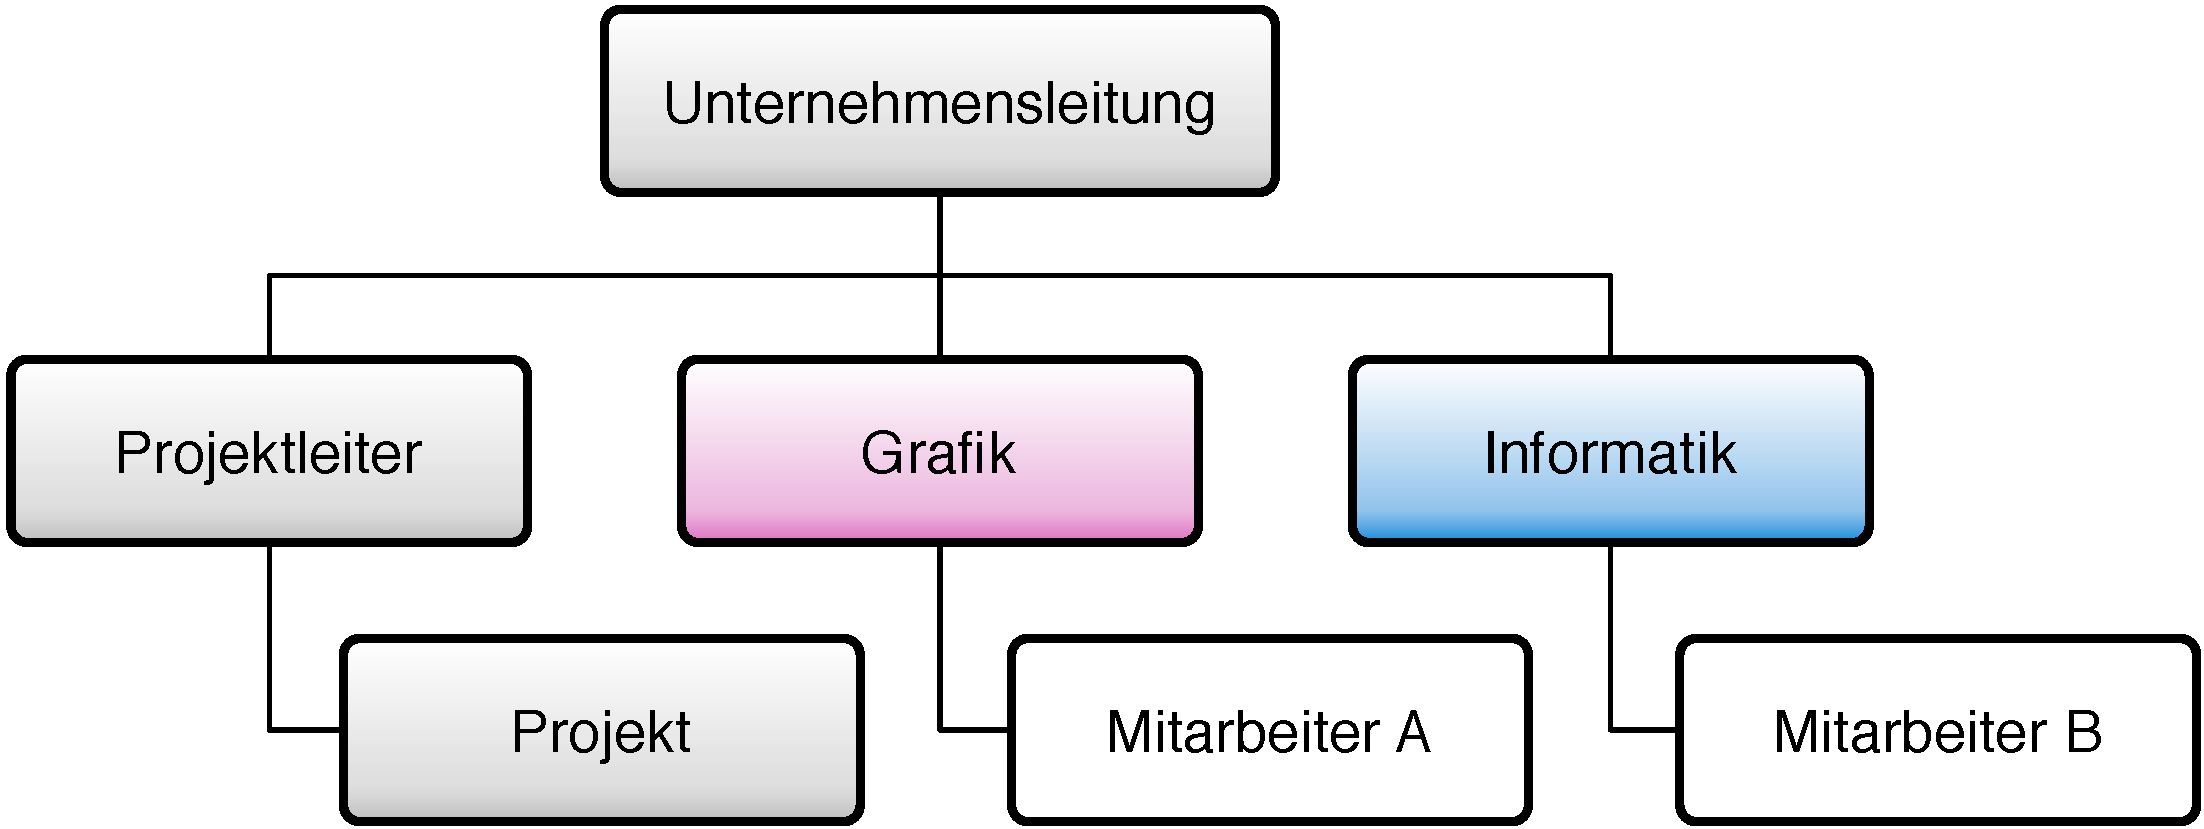
\includegraphics[width=0.7\textwidth,angle=0]{./bilder/loesung/03_projektorganisation.pdf}
\caption[Auftrags-Projektorganisation]{Auftrags-Projektorganisation\footnotemark}
\label{pic:03_projektorganisation}
\end{center}
\end{figure}
\footnotetext{Eigene Darstellung}

Der Projektleiter sucht sich die geeignetsten Mitarbeiter aus, um eine saubere 
Projektplanung erstellen zu können. Gewisse Mitarbeiter können auch nur für die 
Projektplanung, also zum Beispiel als Experten für die Aufwandsschätzung, 
eingeplant werden. Es ist wichtig, dass zu diesem Zeitpunkt noch keine 
Ressourcenplanung erstellt wird. Ist zu diesem Zeitpunkt auch nicht möglich,
da noch keine Projektplanung existiert.

Der Projektleiter eröffnet nun das Projekt im Projektmanagement Tool 
(\textbf{\addtocounter{icounter}{1}AI\arabic{icounter}}) mit einer fortlaufenden
Projektnummer und einer eindeutigen Projektbezeichnung, damit die Aufwände
der Projektplanung bereits auf das Projekt rapportiert werden können.

\subsection{Projektplanung}
In der Grafik \ref{pic:02_02_projektplanung} ist der Ablauf der Projektplanung 
ersichtlich. Als erstes überprüft und sammelt der Projektleiter alle nötigen
Unterlagen, die zur Planung des Projektes notwendig sind (\textbf{3.5}). Falls
noch Unterlagen oder Informationen von Seiten des Kunden fehlen (\textbf{3.6})
fordert er diese beim Kunden ein (\textbf{4.1}). Sobald alle Informationen
vorhanden sind, werden die Arbeitspakete zusammen mit den Mitarbeitern und 
Experten erstellt (\textbf{5.1}). Sind die Arbeitspakete definierte, werden
diese ebenfalls vom Projektleiter in Zusammenarbeit mit den Mitarbeitern und
Experten geschätzt (\textbf{5.2}). Alle Mitarbeiter müssen die hierfür aufgewendete
Zeit auf das Projekt rapportieren (\textbf{\addtocounter{icounter}{1}AI\arabic{icounter}}).

Der Projektleiter erstellt danach die Offerte und macht einen Vorschlag mit
realistischen Timings und Meilensteinen (\textbf{5.4}). Diese bespricht er
mit dem verantwortlichen Partner (\textbf{5.4}). Der Partner wiederum bespricht
danach die Offerte mit dem Kunden (\textbf{5.6}). Wenn weitere Änderungen oder
Anpassungen nötig sind (\textbf{5.7}), nimmt diese der Projektleiter vor. Sobald
die Offerte vom Kunden abgesegnet ist, wird mit der Durchführung des Projektes
begonnen (\textbf{6.1}).

\begin{figure}[htbp]
\begin{center}
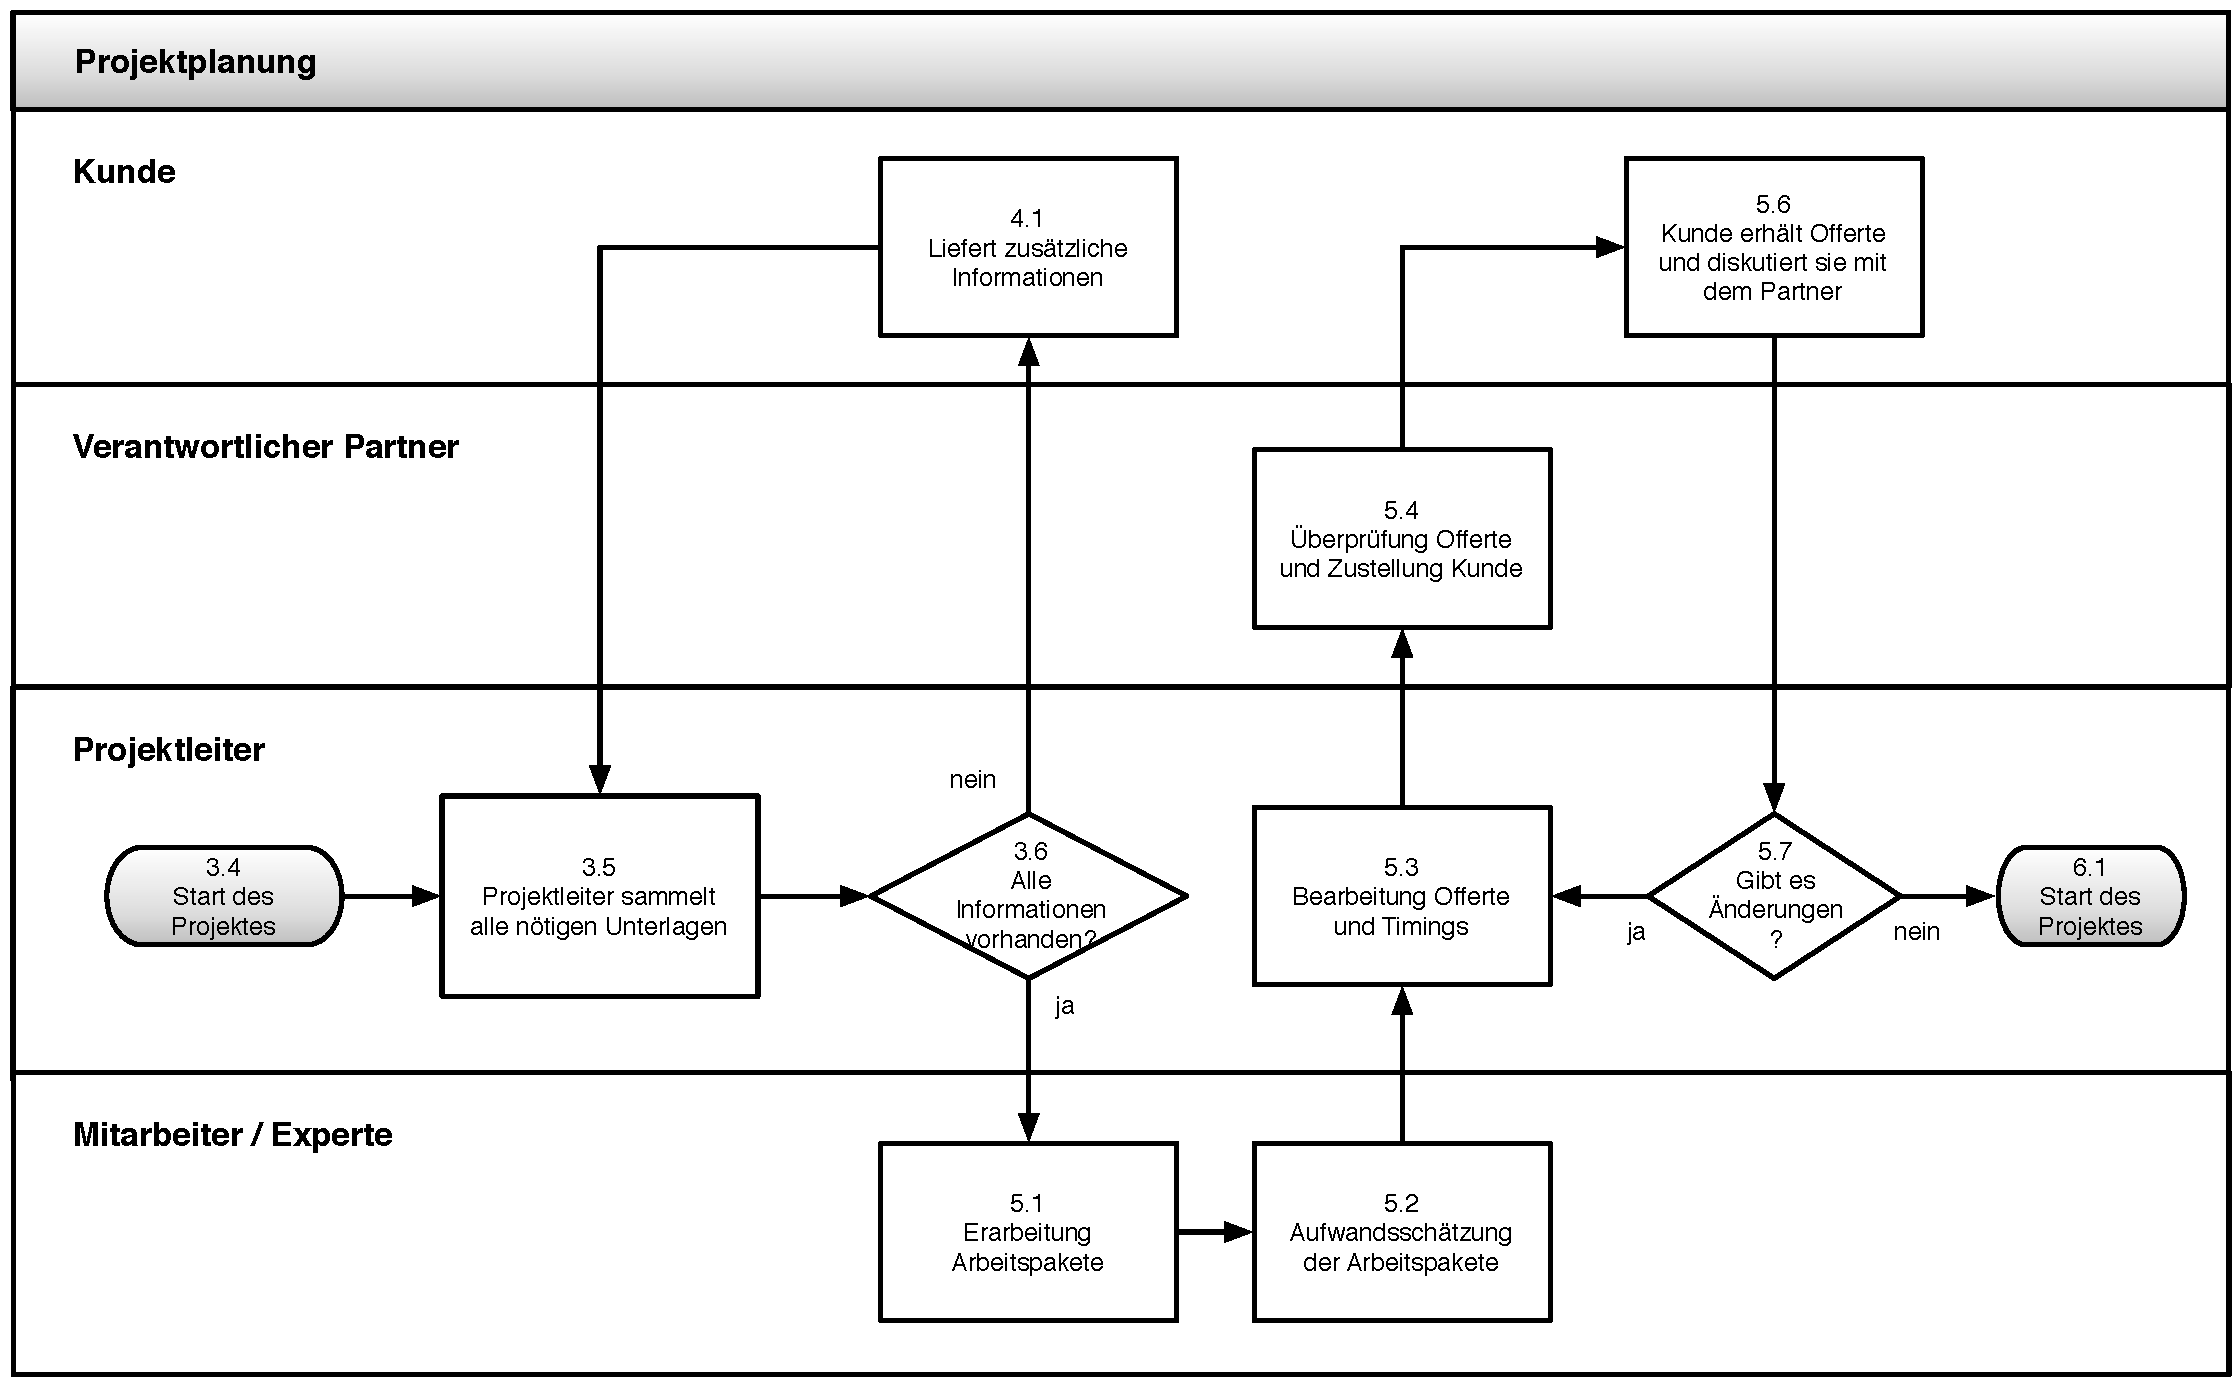
\includegraphics[width=0.99\textwidth,angle=0]{./bilder/loesung/02_02_projektplanung.pdf}
\caption[Ablauf der Projektplanungsphase]{Ablauf der Projektplanungsphase\footnotemark}
\label{pic:02_02_projektplanung}
\end{center}
\end{figure}
\footnotetext{Eigene Darstellung}

\subsubsection{Arbeitspakete}
Die in Zusammenarbeit mit den Mitarbeitern, Experten und, sofern nötig mit dem
verantwortlichen Partner, erstellten Arbeitspakete werden vom Projektleiter
in Todo Listen im Projektmanagement Tool erfasst (\textbf{\addtocounter{icounter}{1}AI\arabic{icounter}}).
Wo sinnvoll und zu diesem Zeitpunkt schon offensichtlich ordnet er den Todos
auch schon die zuständigen Mitarbeiter zu.

\subsubsection{Aufwandsschätzung}
Dank dem Zuziehen der richtigen Mitarbeitern und Experten sollte die Aufwandsschätzung 
realistisch sein. Der zuständige Partner ist verantwortlich diese Schätzung
zu studieren und wenn nötig mit den dafür verantwortlichen Mitarbeitern zu 
diskutieren. Dies ist sehr wichtig, da auf der Aufwandsschätzung die Offerte 
und die Terminplanung basieren.

Zu diesem Zeitpunkt werden auch die nötigen Ressourcen geplant. Im Projektmanagement
Tool werden die nötigen Ressourcen reserviert (\textbf{\addtocounter{icounter}{1}AI\arabic{icounter}}). 
Fall es Konflikte in der Planung einzelner Mitarbeiter gibt, wird zuerst versucht 
ein anderer Mitarbeiter zu wählen. Falls dies nicht möglich ist entscheiden der 
Projektleiter und der verantwortliche Partner ob für dieses Projekt eine zusätzliche 
Ressource geschaffen werden soll, oder man eine Verzögerung des Projektes in Kauf 
nehmen kann. Dies hat einen Einfluss auf die parallel zu erstellende Terminplanung.

\subsubsection{Terminplanung}
Bei der Erstellung der Terminplanung ist es wichtig eine möglichst realistische
Zeitplanung zu erstellen. Diese ist nicht nur von der Aufwandsschätzung abhängig,
sondern kann auch von Kundenvorgaben oder Aufwänden von Drittanbietern beeinflusst
werden. Die erarbeiteten Meilensteine trägt der Projektleiter ebenfalls im
Projektmanagement Tool nach (\textbf{\addtocounter{icounter}{1}AI\arabic{icounter}})
und ordnet, wo sinnvoll, die erstellten Todo Listen den jeweiligen Meilensteinen
zu.

Zu diesem Zeitpunkt kann der Projektleiter auch die geplanten Geldflüsse planen.
Im Projektmanagement Tool erfasst er die genehmigten Offerten, externen Kosten
und Teilzahlungen bzw. Rechnungen (\textbf{\addtocounter{icounter}{1}AI\arabic{icounter}}).
Diese Informationen helfen der Geschäftsleitung eine projektübergreifende und
rollende Liquiditätsplanung zu erstellen.

\subsection{Projektkontrolle}
Während der Durchführung des Projektes kontrollieren der Projektleiter und der 
verantwortliche Partner laufend die Einhaltung der gesetzten Meilensteine und
geplanten Geldflüsse. Alle Mitarbeiter rapportieren während der Durchführung
täglich die aufgewendeten Stunden pro Projekt.

\subsubsection{Terminkontrolle}
Der Projektleiter behält die Abarbeitung der definierten Todo Listen und die
davon abhängigen Meilensteine im Auge. Sobald sich ein Verzug abzeichnet informiert
er frühzeitig den verantwortlichen Partner und in einer gemeinsamen Diskussion,
wenn nötig auch mit den Mitarbeitern des Projektes, wird das weitere Vorgehen
entschieden. Der Projektleiter oder verantwortliche Partner geht anschliessend
proaktiv auf den Kunden zu und informiert ihn über die Veränderungen. Der
Projektleiter passt die Planung im Projektmanagement Tool an.

\subsubsection{Kostenkontrolle}
Der Projektleiter behält auch die auf sein Projekt rapportierten Stunden im Auge.
Er kontrolliert laufend, ob für Arbeiten mehr Stunden als geschätzt aufgewendet
werden. Je nach Grösse der Abweichung informiert er den verantwortlichen
Projektleiter, die wiederum das weitere Vorgehen entscheiden.

Der Projektleiter ist auch dafür verantwortlich, dass die geplanten Rechnungen
rechtzeitig gestellt werden. Die Geschäftsleitung kann diese projektübergreifend
im Projektmanagement Tool kontrollieren und bei Verzögerungen bei den jeweiligen
Projektleitern nachfragen.

\subsection{Projektabschluss}
Sobald alle Todos erledigt sind und alle Meilensteine erreicht wurden kommt
das Projekt in die Projektabschlusssphase. Diese ist in der Darstellung 
\ref{pic:02_03_projektabschluss} abgebildet. Als erstes kümmert sich der
Projektleitung darum, dass die Qualitätskontrolle durchgeführt wird (\textbf{7.2}). 
Sofern Mängel bemerkt werden, werden zusammen mit den Mitarbeitern zusätzliche
Arbeitspakete erstellt (\textbf{8.1}). Wurden keine Mängel entdeckt, erstellt
der Projektleiter den Produktabnahmebericht (\textbf{9.1}). Diesen bespricht er mit dem
verantwortlichen Partner. Dieser wiederum präsentiert dem Kunden die Resultate (\textbf{9.2})
und nimmt das Feedback entgegen (\textbf{9.4}).

\begin{figure}[htbp]
\begin{center}
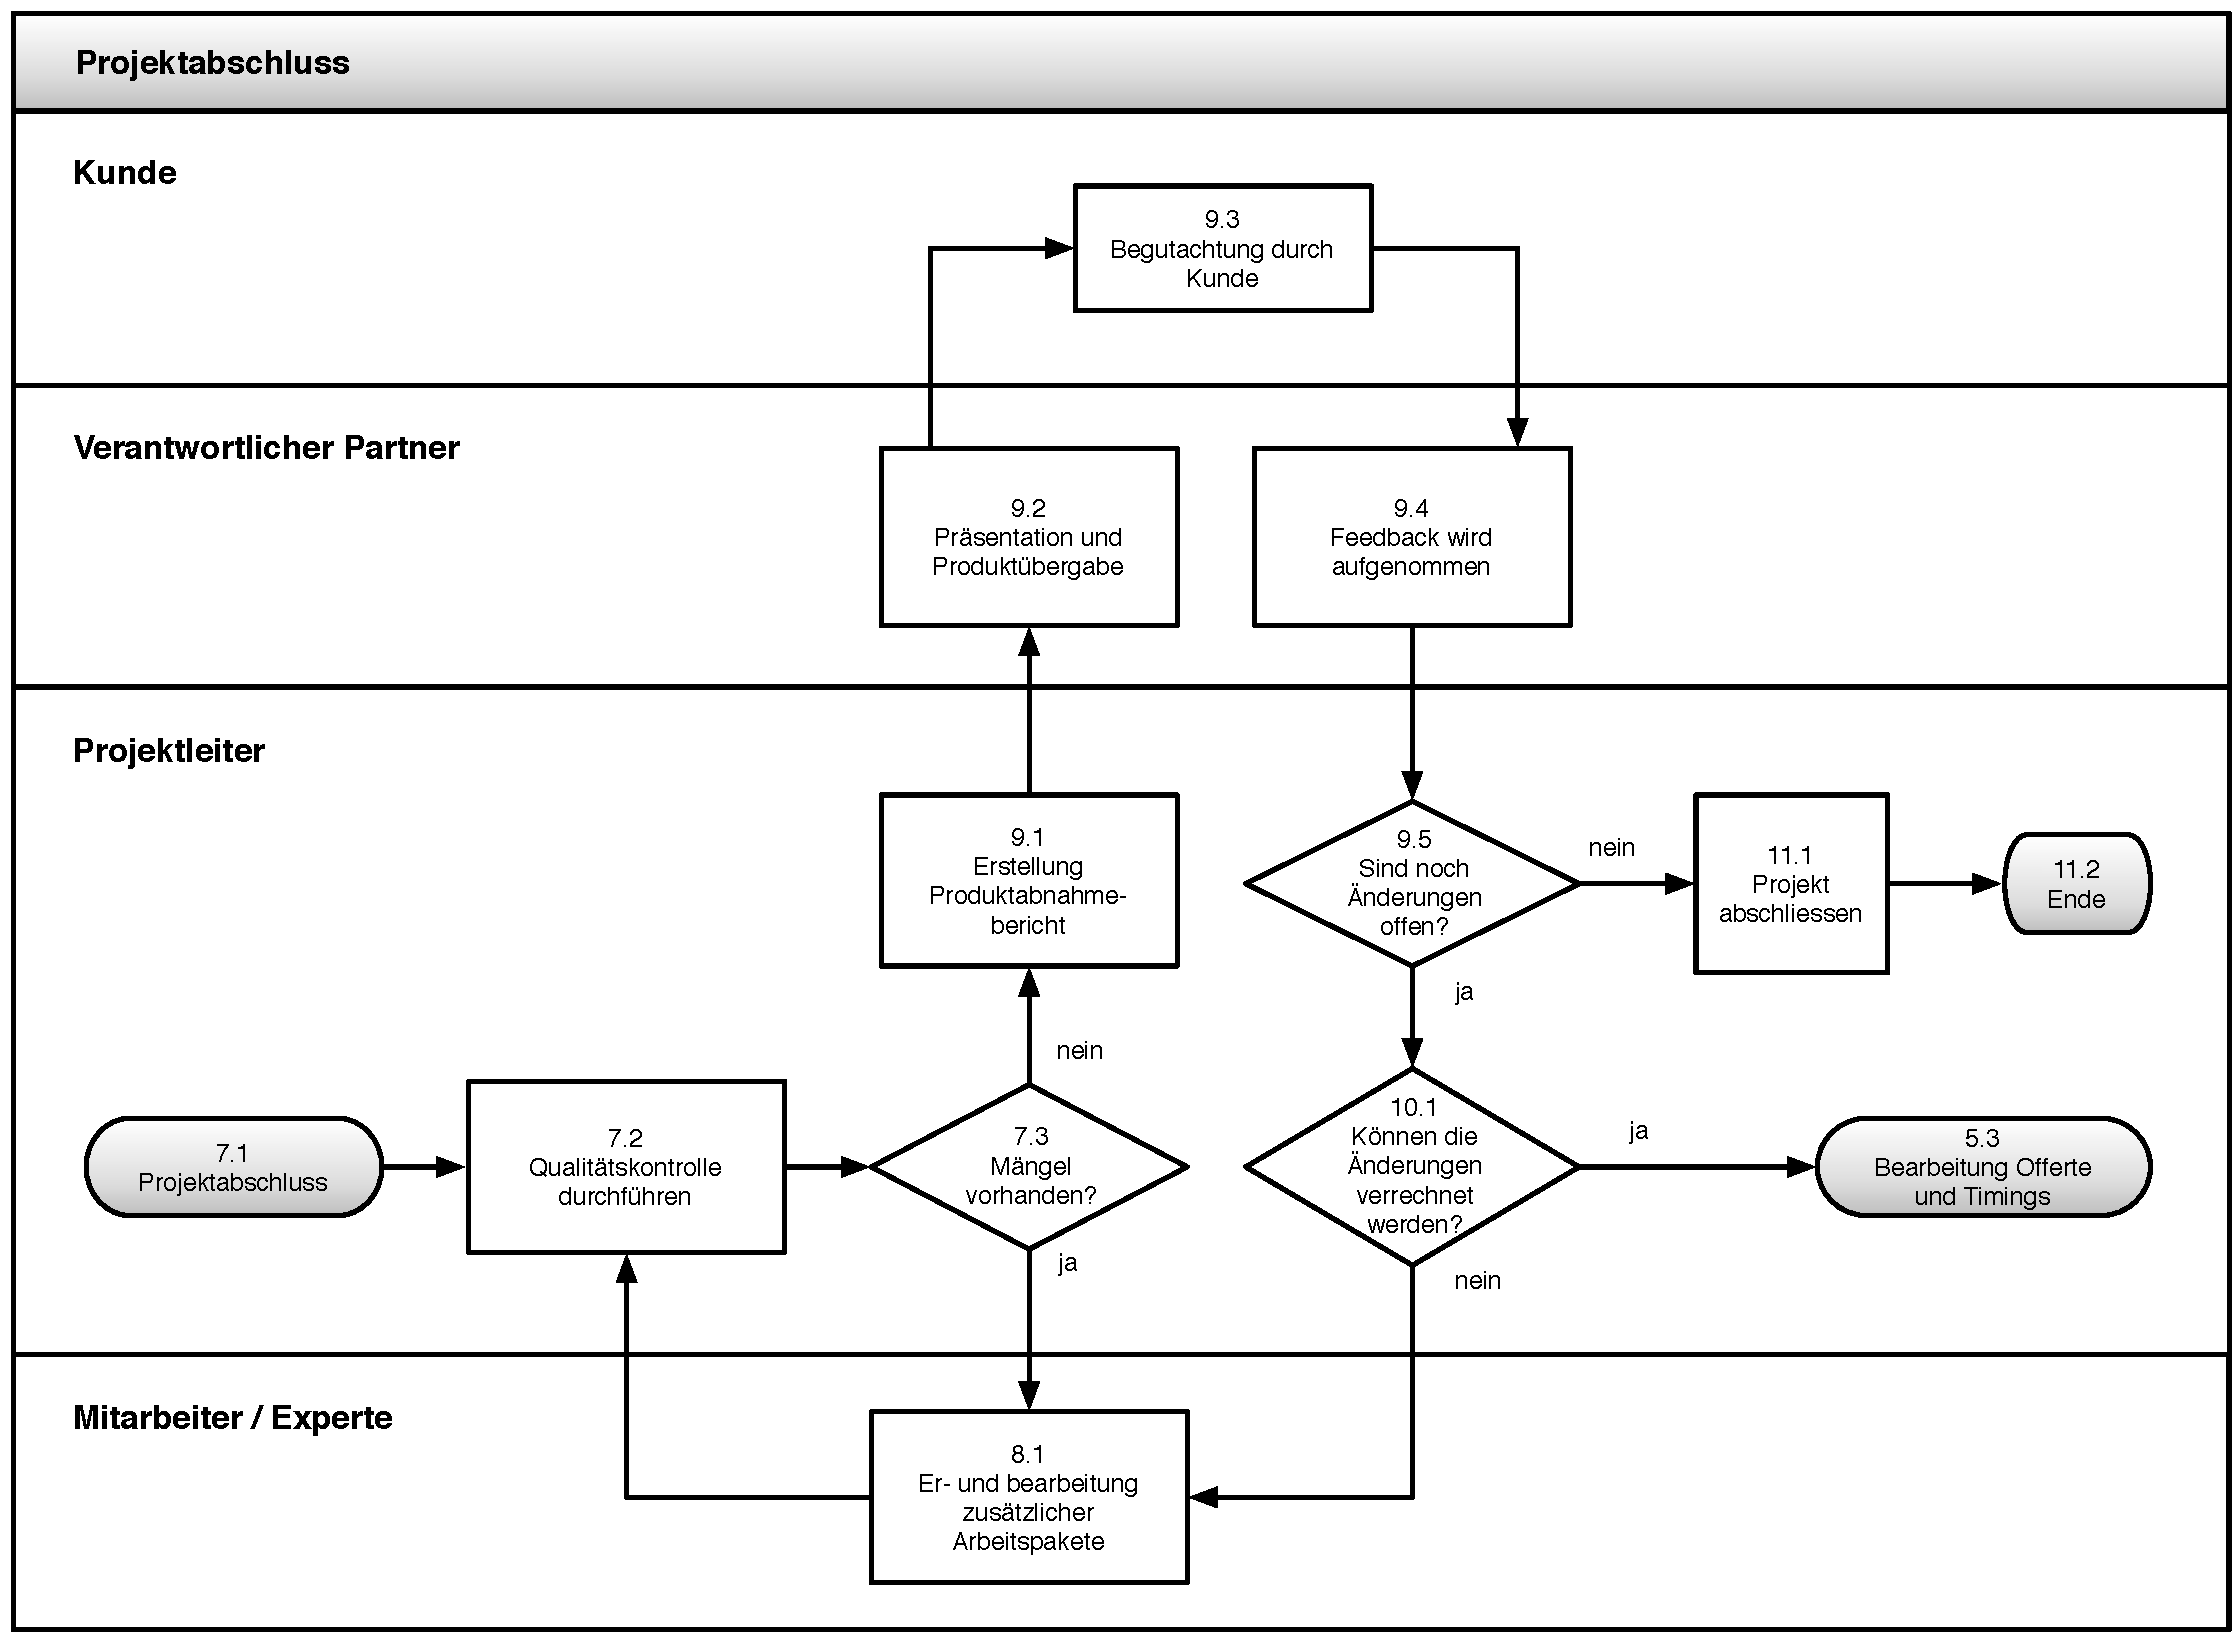
\includegraphics[width=0.99\textwidth,angle=0]{./bilder/loesung/02_03_projektabschluss.pdf}
\caption[Ablauf der Projektabschlusssphase]{Ablauf der Projektabschlusssphase\footnotemark}
\label{pic:02_03_projektabschluss}
\end{center}
\end{figure}
\footnotetext{Eigene Darstellung}

Sind jetzt noch weitere Änderungen offen oder werden zusätzliche Änderungen
gewünscht (\textbf{9.5}) überprüft der Projektleiter zusammen mit dem verantwortlichen
Partner, ob die Anpassungen in den bereits gestellten Offerten enthalten sind, 
oder ob sie zusätzlich verrechnet werden können (\textbf{10.1}). Je nach Fall
passt er die Offerte an (\textbf{5.3}). So oder so werden zusammen mit den 
Mitarbeitern die zusätzlichen Arbeitspakete erstellt (\textbf{8.1}).

Wenn der Kunde vollständig mit dem Resultat zufrieden ist, schliesst der 
Projektleiter das Projekt ab (\textbf{11.1}). Dies beinhaltet das archivieren
aller Projektdaten (\textbf{\addtocounter{icounter}{1}AI\arabic{icounter}}), 
das nachführen des Projektstatus im Projektmanagement Tool und die Reflektionssitzung 
mit allen Projektmitarbeitern. Danach ist das Projekt beendet (\textbf{11.2}).

\subsubsection{Qualitätskontrolle}
Der Projektleiter organisiert in erster Linie die Qualitätskontrolle und sollte
sie nicht selbst durchführen, da er zu nahe am Projekt ist. Entweder übernimmt
dies der verantwortliche Partner oder ein aussenstehender Mitarbeiter.

\subsubsection{Produktabnahme}
Vor der Produktabnahme überprüft der Projektleiter noch einmal den Projektbrief
und alle Offerten. Die Resultate und sonstige Eigenheiten des Projektes hält er
in einem Produktabnahmebericht fest. Dieser bildet die Grundlage für die
Präsentation und Produktübergabe des verantwortlichen Partners und stellt
sicher, dass nichts vergessen gegangen ist.

\subsubsection{Reflektion}
An der Reflektionssitzung müssen alle Mitarbeiter des Projektes inklusive dem
verantwortlichen Partner, damit er die Resultate auch in die Geschäftsleitung 
tragen kann, anwesend sein. Alle positiven und negativen Erfahrungen des Projektes
werden diskutiert. Die Resultate müssen nicht zwingend festgehalten werden,
da die Diskussionen und somit die Verarbeitung der Erfahrungen im Vordergrund 
stehen.